%!TEX TS-program = xelatex
\documentclass[a4paper]{friggeri-cv}
\addbibresource{bibliography.bib}
\usepackage{graphicx} 
\begin{document}
\header{Alexander }{Müller}
       {M.Sc. Candidate Business Informatics}


% In the aside, each new line forces a line break
\begin{aside}
 %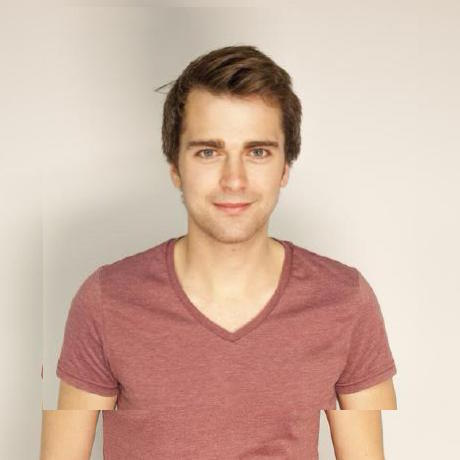
\includegraphics[width=0.7\textwidth]{bild.jpg} 
  \section{about}
  	born 10th January 1989
  	Gütersloh Germany
  	~
   	Neckarpromenade 25/77
    68167 Mannheim
    Germany
    ~
    \href{mailto:alexan.chr.mueller@gmail.com}{mail@alexcmueller.de}
    \href{http://alexcmueller.de}{http://alexcmueller.de}
  \section{languages}
    native German
    fluent English
    intermediate Spanish
  \section{programming}
    Java, Scala
    (EE, Play, Java 8)
    JavaScript
    (Node.js, Angular.js)
    SQL
    (MySQL, SAP HANA)
    NoSQL
    (MongoDB, Redis)
    \section{data analysis}
   	Rapidminer
   	Basic R
   	Spark
   	Weka
   	Stanford Core NLP
   	HANA Predictive Analysis Library
\end{aside}

\section{Interests and Hobbies}

data mining, web mining, natural language processing, ontology matching, linked open data, noSql databases, web development, functional programming, start-ups \\
tennis, running, soccer, politics, European history, movies

\section{Education}

\begin{entrylist}
  \eduentry
    {since 2012}
    {M.Sc. Candidate in Business Informatics}
    {University of Mannheim}
    {Specialization in Data and Web science}
    {Current Grade Point Average of 1.1}
   \entry
    {2013}
    {Exchange Semester in Mexico}
    {ITESM Guadalajara}
    {Language studies}
  \eduentry
    {2009–2012}
    {B.Sc Business Information Technology}
    {DHBW Mannheim in cooperation with SAP SE}
    {Specialization in Software Engineering}
    {Grade Point Average of 1.5}
  \eduentry
    {until 2008}
    {University Entrance Qualification (Abitur)}
    {priv. Gymnasium Marienschule Lippstadt}
    {Specialization in History and Physics}
    {Grade Point Average of 1.4}
\end{entrylist}

\section{Experience}

\begin{entrylist}
  \entry
    {09-10 2014}
    {Burda Bootcamp, München, Germany}
    {Internship}
    {Participant in a rapid prototyping lab (\href{http://burdabootcamp.de}{burdabootcamp.de})}
  \entry
    {02-08 2014}
    {SAP SE, Walldorf, Germany}
    {Working Student}
    {Development of a predictive maintenance model engine based on SAP HANA}
  \entry
    {01–07 2013}
    {University of Mannheim, Chair of PI 1, Germany}
    {Student Research Assistant}
    {Implementation of a SQL-plan parallelizer for XDB}
  \entry
    {2009 - 2012}
    {SAP SE, Walldorf \&  Darmstadt, Germany; Montreal, Canada}
    {Internship}
    {Working in different departments during my studies: (CRM, ByDesign, SAP Research), including an 3-month internship in Montreal, Canada}
\end{entrylist}


\section{Theses, Puplications and Patents}
\begin{entrylist}
	\entry
	 {2015}
    {Masterthesis}
    {University of Mannheim}
    {Working title: An unsupervised Ontology Matching system using Outlier Analysis 	}
	\eduentry
	 {2013}
    {Publication}
    {University of Mannheim}
    {Binnig, Carsten; Salama,Abdallah; Mueller, Alexander C.}
    {XDB: a novel database architecture for data analytics as a service}
	\eduentry
	 {2012}
    {Patent}
    {SAP SE}
    {Doehring, Markus; Drittler, Bernhard; Kieselbach, Oliver; Mueller, Alexander Christian; Zimmerman, Birgit}
	{US20140058789 A1: Process model generation and weak-spot analysis from plain event logs}
	\entry
	 {2012}
    {Bachelorthesis}
    {DHBW Mannheim}
    {Design \& Implementation of a Process Mining Application for the Analysis of Weakspots in Business Processes based on In-Memory Database Technology (Konzeption einer Process Mining Anwendung zur Analyse von Schwachstellen in Geschäftsprozessen auf Basis einer Hauptspeicherdatenbank)}
\end{entrylist}


%\section{patents and publications}

%\printbibsection{misc}{other publications}
%\printbibsection{report}{research reports}

\end{document}
